\documentclass[aps,pra,showpacs,amsmath,amssymb,nofootinbib,longbibliography,superscriptaddress
]{revtex4-1}

%\documentclass[a4paper]{quantumarticle}
%\newcommand{\onlinecite}{\cite}
%\pdfoutput=1
%\usepackage{mcite}
%\usepackage[sort&compress,numbers]{natbib}
%\bibliographystyle{apsrev4-1}


\usepackage[pdftex]{graphicx}
\usepackage[usenames,dvipsnames]{xcolor}
\usepackage{epstopdf}
\usepackage{tikz}    % Include the tikz package for drawing
\usepackage{mathtools}

\usepackage[normalem]{ulem}

\graphicspath{{FIGs/}}

 \usepackage[utf8]{inputenc}
\usepackage[T1]{fontenc}

\usepackage{beramono}
\usepackage{listings}

\usepackage{lmodern}

\usepackage{amssymb,amsmath,amsthm}

\usepackage{bbm}

\usepackage{subcaption}

\usepackage{algorithm}
\usepackage{algpseudocode}

\usepackage{multirow}

\usepackage[justification=raggedright,singlelinecheck=false]{caption}

\DeclareMathAlphabet{\mathbbmsl}{U}{bbm}{m}{sl}

\newtheorem{theorem}{Theorem}
\theoremstyle{definition}
\newtheorem{definition}{Definition}

\theoremstyle{remark}
\newtheorem*{remark}{Remark}

\newtheorem{corollary}{Corollary}[theorem]
\newtheorem{lemma}[theorem]{Lemma}
\renewcommand{\qedsymbol}{$\blacksquare$}

\renewcommand{\lstlistingname}{Code Block}

\newcommand{\patbox}[1]{\vspace{2mm}\noindent\fbox{\parbox{0.47\textwidth}{\hspace{1mm}\parbox{\columnwidth}{\hspace{1mm}\\#1\vspace{1.5mm}}}}\\}

\lstdefinelanguage{julia}%
  {morekeywords={abstract,break,case,catch,const,continue,do,else,elseif,%
      end,export,false,for,function,immutable,import,importall,if,in,%
      macro,module,otherwise,quote,return,switch,true,try,type,typealias,%
      using,while},%
   sensitive=true,%
   alsoother={\$},%
   morecomment=[l]\#,%
   morecomment=[n]{\#=}{=\#},%
   morestring=[s]{"}{"},%
   morestring=[m]{'}{'},%
     literate={é}{{\'e}}1
           {è}{{\`e}}1
           {ù}{{\`u}}1
}[keywords,comments,strings]%

\lstset{%
    language          = julia,
    basicstyle        = \ttfamily,
    keywordstyle      = \bfseries\color{blue},
    numbers           = left,
    numbers           = none,
    stringstyle       = \color{magenta},
    commentstyle      = \color{ForestGreen},
    showstringspaces  = false,
    frame             = single, 
    inputencoding     = latin1,
    breaklines        = true,
    breakatwhitespace = true
}

\newcommand{\FRrefsec}[1]{sec.~\ref{#1}}
\newcommand{\FRreffig}[1]{fig.~\ref{#1}}
\newcommand{\FRrefeq}[1]{eq.~\ref{#1}}

\newcommand{\ENrefsec}[1]{Sec.~\ref{#1}}
\newcommand{\ENreffig}[1]{Fig.~\ref{#1}}
\newcommand{\ENrefeq}[1]{Eq.~\ref{#1}}



\newcommand{\Ham}{\hat{\mathcal{H}}}
\newcommand{\Spin}{\hat{S}}
\newcommand{\A}{\hat{A}{}}
\newcommand{\B}{\hat{B}{}}
\newcommand{\M}{\hat{M}}
\newcommand{\densmat}{\hat{\rho}}
\newcommand{\U}{\hat{U}{}}
\newcommand{\D}{\hat{D}{}}
\newcommand{\V}{\hat{V}{}}
\newcommand{\X}{\hat{X}{}}
\newcommand{\W}{\hat{W}{}}
\newcommand{\bigOmega}{\hat{\Omega}{}}
\newcommand{\bigLambda}{\hat{\Lambda}{}}
\newcommand{\bigGamma}{\hat{\Gamma}{}}


\newcommand{\I}{\hat{I}}
\newcommand{\0}{\hat{0}}

\newcommand{\x}{\mathbf{x}}
\newcommand{\dx}{\mathrm{d}\mathbf{x}}

\newcommand{\Z}{\mathcal{Z}}

\newcommand{\dt}{\mathrm{d}t}









   \newenvironment{xabstract}
{\onecolumngrid
    \list{}{%
        \setlength{\leftmargin}{.5in}% 
        \setlength{\rightmargin}{\leftmargin}%
        }%
        \item\relax}
        {\endlist}




\usepackage[compat=1.1.0]{tikz-feynman}




%\usepackage{chngcntr}


\usepackage[hidelinks]{hyperref}


\begin{document}

% \title{Honours Thesis Project Proposal - Simulation of Squeezed Light Generation in an Optical Resonator}
% \author{Aaron Dayton}

% \maketitle


\begin{center}
    \textbf{\Large Honours Thesis Project Proposal - Simulation of Squeezed Light Generation in an Optical Resonator} \\ % Your title
    \vspace{0.5cm} % Space between title and author
    \Large Aaron Dayton \\ % Your name
    \vspace{0.3cm} % Space between author and date
    \today \\ % Current date
\end{center}


\section{Introduction}

As quantum technologies advance, the need for quantum networks grows rapidly. With proposed applications like quantum key distribution and quantum computation, a way to reliably transmit quantum information with low losses is required to obtain the maximal benefit from these systems. An additional challenge is to surpass the standard quantum limit (SQL) which imposes a limitation on quantum measurement precision according to the uncertainty principle. So there are two needs in the current landscape of quantum technologies which will be worked towards by this project: to transmit/transfer quantum information reliably, and to surpass the SQL for optical quantum signals.


Optical squeezed states are states in which an electromagnetic field has its uncertainty with respect to one canonical variable increased (either phase or amplitude) while the uncertainty in the canonical conjugate variable is decreased (either amplitude or phase, respectively) such that the uncertainty principle is observed. This allows for precision measurements of the low-uncertainty variable to be made which surpass the SQL.

The non-linear optical process of four wave mixing (FWM) has been shown to be able to produce squeezed states \cite{FWMSS}. It has also been shown that if FWM is performed using three-level atoms ($\Lambda$-system), then entanglement can be produced \cite{FWMIE}. FWM can also convert optical frequencies \cite{FWMIE}. Additionally, quantum fluctuations for three-level atoms can be controlled in resonant cavities using electromagnetically induced transparency (EIT) \cite{CCQF}.

These ideas will be built upon to computationally model the dynamics of a resonant cavity filled with three-level atoms in order to produce squeezed states through FWM and cavity EIT. This project works towards quantum networking as frequency conversion for quantum entangled signals could allow for quantum information to be transferred through fibre optic cables at a low-loss frequency, and towards surpassing the SQL by finding the conditions in which squeezed states can be produced given a system with a set of tunable parameters.

\section{Proposed Work}

This project requires firm understanding of optical non-linearities, electromagnetically induced transparency, squeezed states, three-level atoms, four wave mixing, continuous variable entanglement, the Fock basis, and the master equation. These topics will be learned in the first stage.

The system to be modelled is depicted in Fig.~\ref{SphericalResonator}. If for the two output beams we have $\omega_a \neq \omega_b$, then the system will produce what is called a two-mode squeezed state; if $\omega_a = \omega_b$, then the system will produce a single mode squeezed state. This project will focus on the production of a single-mode squeezed state. The purpose of the spherical resonator is to enhance the single-mode output field produced in this process such that photons can be detected above the shot-noise level. The system will be modelled by setting up a Hamiltonian in the Fock basis for photons.

\begin{figure}[h!]
    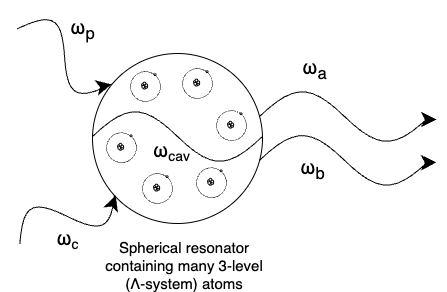
\includegraphics[width=0.5\columnwidth]{SphericalResonator.png}
    \caption{System involving two continuous electromagnetic input beams at frequencies $\omega_p$ and $\omega_c$ which undergo a four wave mixing process within a spherical resonator tuned to frequency $\omega_{cav}$ filled with cooled three-level atoms to produce output fields at frequencies $\omega_a$ and $\omega_{b}$, respectively.}
    \label{SphericalResonator}
\end{figure}


Computations will then be performed which find a steady state density matrix $\rho$ of the Lindblad master equation dictating the time evolution of the system
\begin{equation}
    \frac{d \rho}{\dt} = - \frac{i}{\hbar} [H, \rho] + \sum_i \gamma_i \left( L_i \rho L_i^{\dagger} - \frac{1}{2} L_i^{\dagger} L_i \rho - \frac{1}{2} \rho L_i^{\dagger} L_i \right)
\end{equation}
where $L_i$ are operators describing the dissipative dynamics of the system. i.e. the goal is to solve for when $\dot{\rho} = 0$. Parameters such as, but not limited to, laser intensity and atomic density may be varied across computations.

Results will be analyzed to find when the desired single-mode squeezed states would theoretically be produced. Validation of these results would then be attempted in future experiments.


\section{Timeline}

The timeline for this project can be broken down into five main stages. First, relevant background knowledge must be obtained. Second, the problem must be formulated mathematically. Third, the modelled system must have computations performed to find relevant results. Fourth, the results must be analyzed to find the system conditions which promote optimal squeezed state generation. Fifth, thesis finalization. The thesis will be written concurrently with these steps as they occur. These stages are outlined with proposed due dates in the following table.

\begin{center}
    \begin{tabular}{ |p{4cm}||p{10cm}|p{3cm}|  }
        \hline
        \multicolumn{3}{|c|}{Project Timeline} \\
        \hline
        Stage &  Description & Proposed due date\\
        \hline
        \raggedright Obtain background knowledge & Learn about optical non-linearities, electromagnetically induced transparency, squeezed states, three-level atoms, four wave mixing, continuous variable entanglement, the Fock basis, and the master equation. & September 30, 2025\\
        \hline
        Mathematical formulation & Set up the system Hamiltonain and an equation for the time evolution dynamics using the master equation. & November 30, 2025\\
        \hline
        Perform computation and obtain results & Find steady states of the Hamiltonain for the master equation using computational methods over various system parameters such as detunings. & January 31, 2026\\
        \hline
        Result analysis & Analyze data and find when optimal squeezed states are produced at the desired frequencies (in time for Honours fest). & February 15, 2026\\
        \hline
        Thesis finalization & Complete writing and editing of the thesis to prepare it for submission. & April 2, 2026\\
        \hline
    \end{tabular}
\end{center}



\bibliography{refs}


\end{document}